\documentclass[a4paper]{article}

\usepackage[T1]{fontenc}
\usepackage[utf8]{inputenc}
\usepackage{tikz}
\usepackage{textcomp}

\begin{document}
\thispagestyle{empty}

\begin{tikzpicture}[remember picture,overlay]

\node [align=center] at (current page.north) % upper
      {\begin{tikzpicture}[remember picture, overlay]
	  \fill[fill=blue!30] (-10,0) rectangle (10,-0.5);
	  \node[anchor=north] at (0,-0.5) {\Large\textit{Getting kudos on A03}};
      \end{tikzpicture}};
      
\node [align=center] at (current page.center) % dragon
      {\begin{tikzpicture}[remember picture, overlay]
          \node[anchor=center,align=center] at (0,5)
               {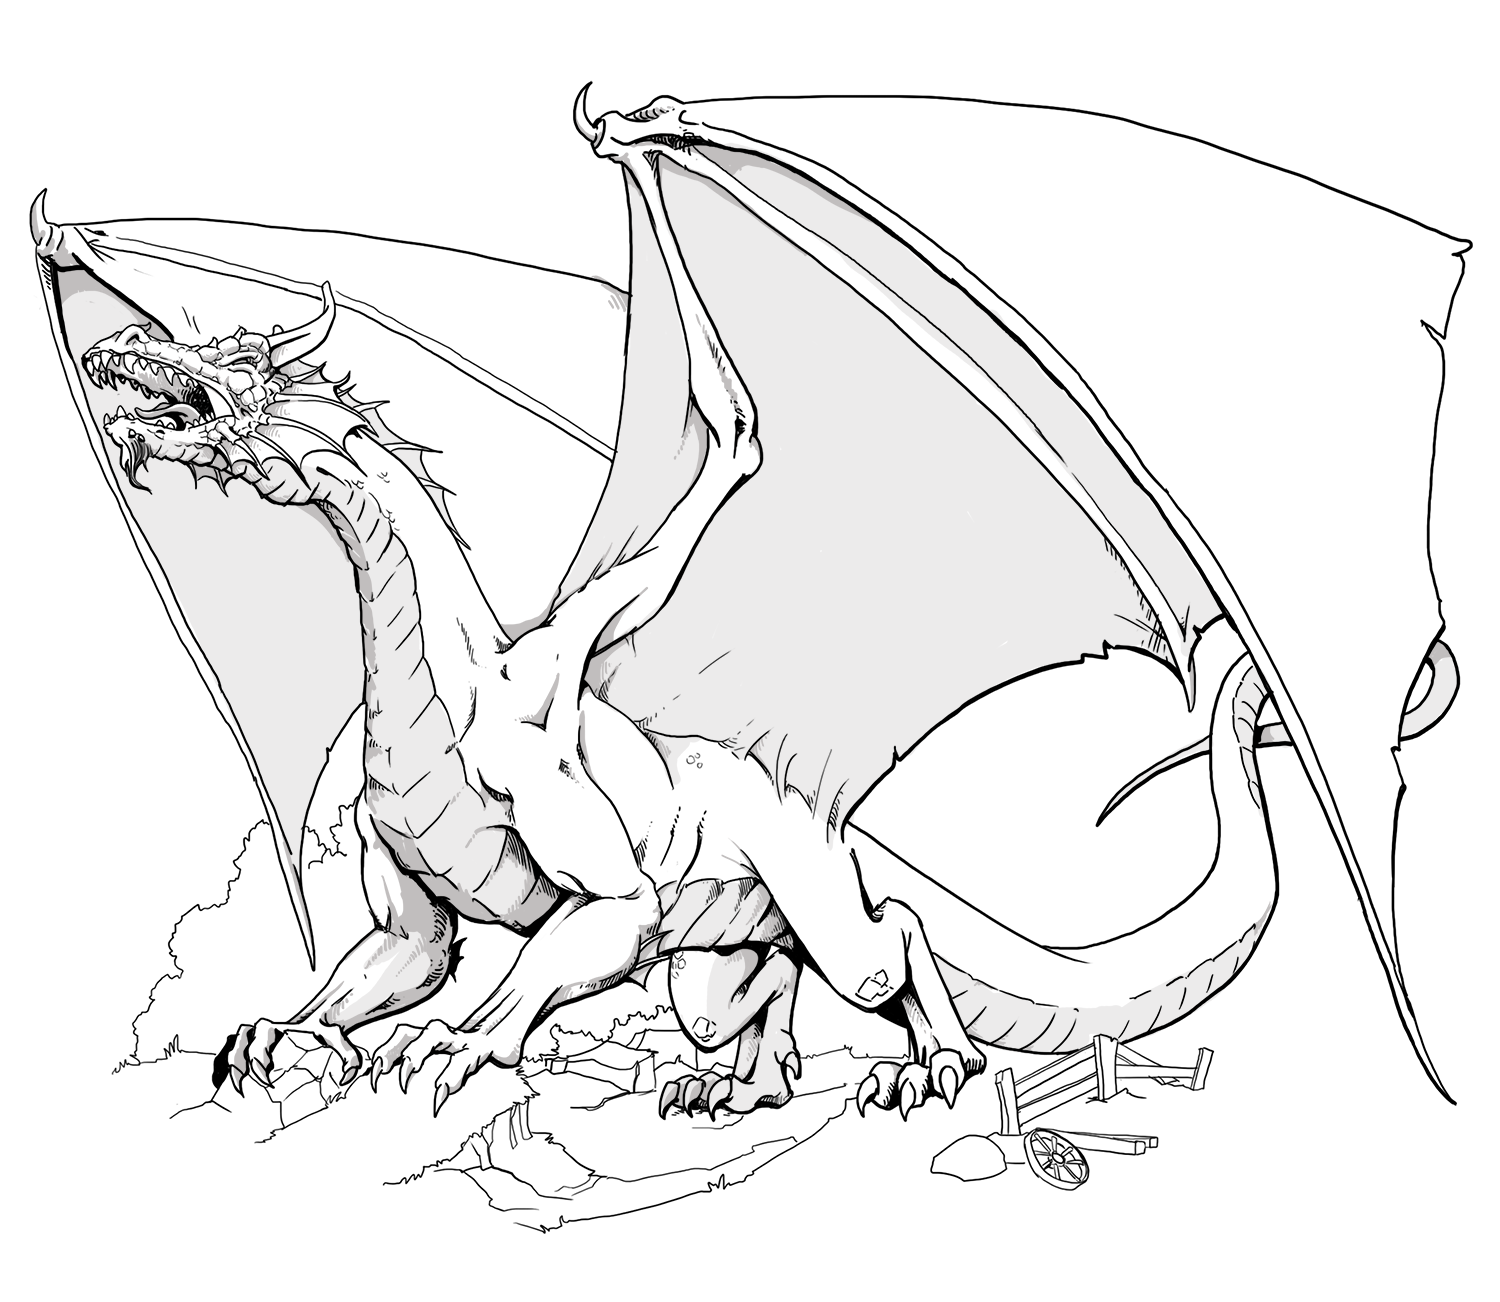
\includegraphics[width=1.5\textwidth]{dragon.png}};
               % from https://commons.wikimedia.org/wiki/File:DnD_Dragon.png
      \end{tikzpicture}};

\node [yshift=-5cm] at (current page.center) % title
      {\begin{tikzpicture}[remember picture, overlay]
          \fill[fill=blue!30] (-10,-5) rectangle (10 ,1);
          \node[align=center] at (0,-2)
               {\resizebox{1.57\linewidth}{!}{\Huge\textbf{Writing}}};
	       \node[anchor=east,align=right] at (10,-5.5) {\Huge\color{black}\textit{very good fanfiction}};
      \end{tikzpicture}};

\node [shift={(-5cm,-5cm)}] at (current page.north east) % Revision 2
      {\begin{tikzpicture}[remember picture, overlay]
          \draw[fill=black] (0,5) -- (1.5,5) -- (5,1.5) -- (5,0) -- cycle ;
          \node[inner sep=0pt,rotate=-45] (rev) at (2.9,2.9) {\huge\color{white}\textbf{Revision 2}};
      \end{tikzpicture}};

\node [align=center] at (current page.south) % bottom
      {\begin{tikzpicture}[remember picture, overlay]
          \node[anchor=south west, align=left] at (-10,0.5)
               {\resizebox{.3\linewidth}{!}
                 {\Huge\color{black}
                   \textbf{G\color{blue!30}'\color{black}ARGLE\textsuperscript{\Large{\textregistered}}}}};
               \node[anchor=south east, align=right] at (10,0.5) {\Huge\color{black}\textbf{Loeka}};
      \end{tikzpicture}};

\end{tikzpicture}

\end{document}
